\documentclass{beamer}
\usetheme{metropolis} % Use metropolis theme





\title{ECON 3818: Introduction to Statistics with Computer Applications}
%\subtitle
\date{\today}
\author{Kyle Butts}

\definecolor{blue}{RGB}{0,114,178}
\definecolor{red}{HTML}{EB0E09}
\definecolor{yellow}{RGB}{240,228,66}
\definecolor{green}{RGB}{0,158,115}
\definecolor{maroon}{HTML}{AF3335}
\definecolor{purple}{HTML}{7E90B8}

\definecolor{mybackground}{HTML}{ECECEC}
\setbeamercolor{background canvas}{bg= mybackground}

\definecolor{buff-gold}{HTML}{CFB87C}
\definecolor{buff-grey}{HTML}{565A5C}
\definecolor{buff-lightgrey}{HTML}{A2A4A3}
\definecolor{buff-black}{HTML}{000000}

\setbeamercolor{alerted text}{fg=buff-gold!80!black}
\setbeamercolor{frametitle}{bg=buff-black}
\setbeamercolor{title}{fg=buff-grey}
\setbeamercolor{button}{bg=buff-gold}

% Allow to remove indent w/ \begin{itemize}[leftmargin= *]
\usepackage{enumitem}
\setlist[itemize]{label= \textbullet}

% \usepackage[libertine]{newtxmath}
\usepackage{longtable}
\usepackage{booktabs}
\usepackage{enumitem}




\begin{document}

% Title Page ---------------------------------------
\maketitle



\begin{frame}{Review}
	Suppose that the population of statistic students' test scores is $X \sim N(80, 9)$. Consider a sample of size 36.

	\begin{itemize}
		\item What is the probability of observing a student with test score greated than $90\%$?
		
		\item What is the distribution of the sample average test score $\bar{X}$? 

		\item Describe what a sample distribution of average test scores is.
		
		\item What's the probability that a sample average test score of size $n = 36$ is less than 75?		
		
		\item Suppose a sample average test score of size $n = 36$ is $\bar{X} = 78$. What is the 95\% confidence interval associated with this sample mean?
	\end{itemize}

\end{frame}

\begin{frame}
\end{frame}

\begin{frame}
\end{frame}


% Chapter 18 ---------------------------------------
\section{Chapter 18: Inference in Practice}

\begin{frame}{Making Inferences}
	So far we have discussed two ways to make inferences about the parameter using our estimate 
	\begin{itemize}
		\item Confidence intervals
		\item Hypothesis testing
	\end{itemize}
\end{frame}

\begin{frame}{Cautions about Confidence Intervals}
	Important to note that the \alert{margin of error} doesn't cover all errors
	\begin{itemize}
		\item address only random sampling errors, not other issues such as undercoverage, nonresponse, etc.
	\end{itemize}
\end{frame}

\begin{frame}{Choosing Sample for Confidence Intervals}
	
	\begin{itemize}
		\item As we mentioned, it is important to make sure we have a Simple Random Sample when constructing a confidence interval. 
		
		\item Additionally, the researcher can determine the number of observations required in the sample in order to achieve a desired margin of error. 
		
		\[
			m = z^* \frac{\sigma}{\sqrt{n}} \pause \implies n=\big(\frac{z^*\sigma}{m}\big)^2,
		\]
		where m is the desired margin of error, and z* is the z-score associated with the confidence interval level
	\end{itemize}
\end{frame}

\begin{frame}{Example}
	Say we are recording tip size of patrons when a waiter writes a message on the receipt. We know $\sigma=2$. We want to estimate the mean percentage tip $\mu$ for patrons who receive the message within $\pm$ 0.5 with 90\% confidence. How many patrons must we observe?
	\vskip.2in
	$$
		n = \left( \frac{z^*\sigma}{m} \right)^2 \implies n = \left(\frac{1.645\cdot 2}{0.5} \right)^2 = 43.3 
		$$
\end{frame}

\begin{frame}{Cautions about Hypothesis Testing}
	These tests of significance depend on: 

	\begin{itemize}
		\item The alternative hypothesis
		\item The sample size
	\end{itemize}
\end{frame}

\begin{frame}{Planning for Hypothesis Testing}
	\begin{itemize}
		\item Our choice of level of significance, $\alpha$, depends on whethere we REALLY want not wrongly reject $H_0$ or if we REALLY don't want to fail to reject $H_0$
	\end{itemize}
\end{frame}

\begin{frame}{Types of Error}
	
	In any statistical test there are four possible outcomes:

	\begin{center}
		\begin{tabular}{|c|c|c|}
			\hline
			& $H_0$ true & $H_a$ true \\
			\hline
			Reject $H_0$ & Type I Error & Correct \\
			\hline
			Fail to Reject $H_0$ & Correct & Type II Error \\
			\hline
		\end{tabular}
	\end{center}
\end{frame}


\begin{frame}{Type I Error}
	\alert{Type I Error}: Rejecting a true null hypothesis
	
	\begin{itemize}
		\item We reject $H_0$, even though $H_0$ is true
		      
		\item We wrongfully decide against the null, when it is actually true 
		      \begin{itemize}
		      	\item False-positive on a strep throat test
		      	      \begin{itemize}
		      	      	\item $H_0$: You do not have strep throat
		      	      \end{itemize}
		      \end{itemize}
		      
		\item Denote the probability of a type I error as $\alpha$
		
	\end{itemize}
	
	Since our null hypothesis is \textit{typically} that there is no effect, a type I error \textit{typically} says there is an effect when in reality there is not
\end{frame}

\begin{frame}{Type II Error}
	\alert{Type II Error}: Failing to reject a false null
	
	\begin{itemize} 
		\item We fail to reject $H_0$, even though $H_0$ is false
		      
		\item We do not reject the null when the null is actually false
		      \begin{itemize}
		      	\item False-negative on strep-throat test
		      	      \begin{itemize}
		      	      	\item $H_0$: You do not have strep throat
		      	      \end{itemize}
		      \end{itemize}
		      
		\item Denote the probability of type II error as $\beta$

	\end{itemize}
	
	Since our null hypothesis is \textit{typically} that there is no effect, a type II error \textit{typically} says there is not an effect when in reality there is something different going on 
\end{frame}

\begin{frame}{Type I and II Errors}
	\centering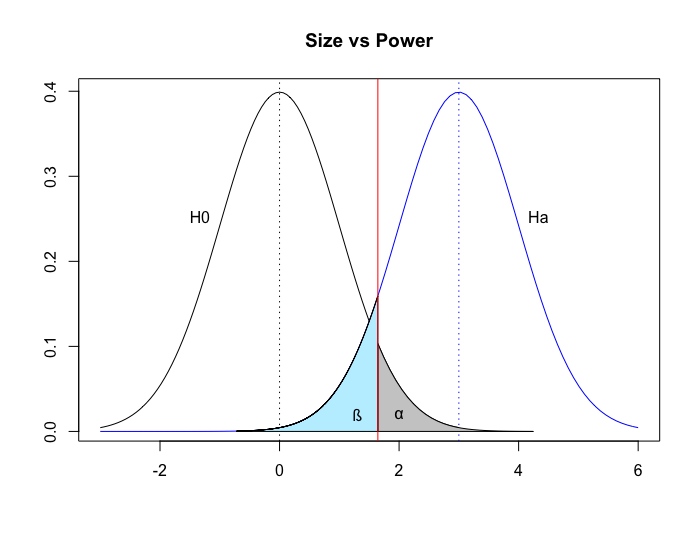
\includegraphics[width=.8\textwidth]{sizevspowerab.png}
\end{frame}

\begin{frame}{Clicker Question}
	Suppose we have the following hypothesis test:
	
	\begin{center}
		\begin{itemize}
			\item[$H_0$:] Taking multivitamins does not impact your running speed
			\item[$H_1$:] Taking multivitamins \textit{will increase} your running speed
		\end{itemize}
	\end{center}

	If we make the claim ``Taking vitamins in the morning will increase your running speed'' and it is not true, we have committed a:
	
	\begin{enumerate}[label=(\alph*)]
		\item Type I error
		\item Type II error
	\end{enumerate}
\end{frame}

\begin{frame}{Errors in Hypothesis Testing}
	How do these errors happen?
	\begin{itemize}
		\item Our conclusions are based on sample data and probabilities 
		      \begin{itemize}
		      	\item We could have an unusual sample
		      	\item We do not have enough information (sample size)
		      	\item We do not choose to be very rigorous ($\alpha$)
		      \end{itemize}
		      
		\item In particular we control
		      \begin{itemize}
		      	\item Type I error is determined by the significance of the test, $\alpha$
		      	\item Type II error depends on the distribution when the null is false
		      	      \begin{itemize}
		      	      	\item However, we can mitigate it by increasing the sample size
		      	      \end{itemize}
		      \end{itemize}
	\end{itemize}
\end{frame}

\begin{frame}{Size of a Test}
	Now that we've defined Type I error, lets define size:
	\vskip.25in
	\begin{definition}[Size]
		\vspace{5mm}
		The \alert{size} of a test, $\alpha$, is the probability of making a Type I error. 
		
		Given a null hypothesis $H_0: \theta = \theta_0$, a test statistic, $\hat{\theta}$, and a rejection region R, 
		$$\alpha = P(\text{Type I Error})=P(\hat{\theta}\in R \ \vert \ \theta=\theta_0)$$
	\end{definition}
\end{frame}

\begin{frame}
	
	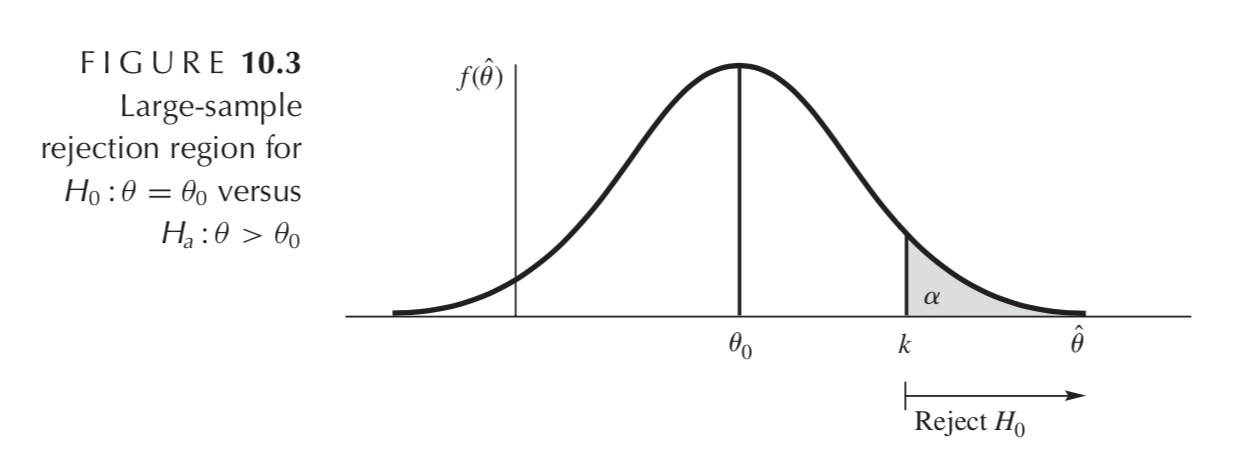
\includegraphics[width=\textwidth]{onesidedtest}
	\begin{center}
		{\tiny Source: \textit{Mathematical Statistics with Applications, Wackerly et al.}}
		\[ R = \{ \widehat{\theta} \ \vert \ \widehat{\theta} > k \} = (k, \infty) \]
	\end{center}
\end{frame}

\begin{frame}{Calculating the Size of a Test}
	How do we actually calculate $\alpha$?   Let's suppose we have $n=16$ and $\sigma=1$, and we want to test $H_0$: $\mu=3$ vs. $H_a$: $\mu > 3$.   
	
	Given a rejection region of $R=\{ \bar{X} \ \vert \ \bar{X} > 3.41 \}$, what is $\alpha$?
			 
	\pause \[
		\alpha = P( \widehat{\theta} \in R \ \vert \ \theta = \theta_0 ) = \left.P(\bar{X} > 3.41\right \ \vert \ {\mu=3}) 
	\]

	\[ 
		= P\left(\frac{\bar{X} - \mu}{\sigma / \sqrt{n}} > \frac{3.41 - 3}{1/\sqrt{16}}\right) = Pr(Z > 1.64)
	\]
	
	\[ = 0.05 \]
			
\end{frame}
	

\begin{frame}{Choosing Size}
	Note that we have to pick \underline{either} the rejection region or the size
	\begin{itemize} 
		\item This is because choosing one determines the other
	\end{itemize}
	
	\begin{itemize}
		\item We generally pick a size and calculate the rejection region based off that size
		      \begin{itemize}
		      	\item Because the size is the probability of a rejecting a true null, by choosing $\alpha$ we are choosing how much we are willing to risk \textit{incorrectly} rejecting the null hypothesis
		      	
				\item Higher $\alpha$ will mean more of the sample statistics are in the rejection region, meaning a higher risk of rejecting the null even though it's true 
		      \end{itemize}
	\end{itemize}
\end{frame}

\begin{frame}{Power of a Test}
	While size deals with Type I Errors, power deals with Type II.

	\begin{definition}[Power]
		\vspace{5mm}
		The \alert{power} is the probability of correctly rejecting a false null, or 1 - P(Type II Error)
		
		\[ \text{Power} = 1 - P(\text{Type II Error}) \]
	\end{definition}

	Intuitively, power is the likelihood of detecting a false null using your test statistic.
\end{frame}

\begin{frame}{Power and Probability of Type II Errors}
	A Type II error is the probability of failing to reject a false null

	$$P(\text{Type II})=P(\bar{X} \notin R \ \vert \ \mu \neq \mu_0)$$
	
	The \alert{Power} is the probability of correctly rejecting a false null

	$$Power=P(\bar{X} \in R \ \vert \ \mu \neq \mu_0)$$
	
	You can think of power as the probability of \textit{not making a Type II error}
	
	You can calculate power by doing $1 - P(\text{Type II})$ or by calculating the power directly.
\end{frame}

\begin{frame}{Type I and II Errors}
	\centering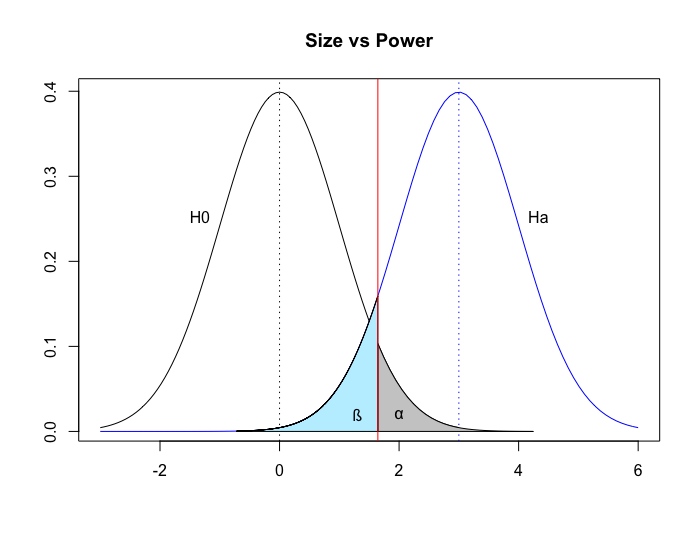
\includegraphics[width=.8\textwidth]{sizevspowerab.png}
\end{frame}

\begin{frame}{Power}
	\centering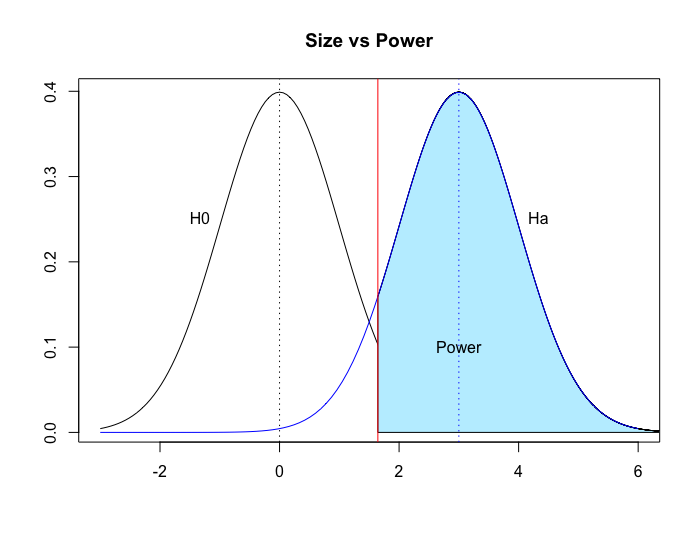
\includegraphics[width=.8\textwidth]{sizevspowerapower.png}
\end{frame}

%\begin{frame}{Calculating the Power of a Test}
%To calculate the power, we first calculate the probability of a Type II Error.
%\vskip.2in
%Given a null $H_0=\theta_0$, a test statistic, $\hat{\theta}$, and rejection region R:
%$$P(\text{Type II Error})=P(\hat{\theta} \notin R  \ \vert \  \theta \neq H_0)$$
%\end{frame}

\begin{frame}{Calculating the Power of a Test}
	Back to previous example, where $n=16$, $\sigma=1$, and $R=\{ \bar{X}  \ \vert \  \bar{X} > 3.41 \}$. And we are testing $H_0: \mu=3$ vs. $H_1: \mu>3$:
	
	Power can be calculated in two ways: 
	
	\begin{itemize}
		\item Power = P(reject $H_0 \ \vert \ H_0$ false) = $P(\bar{X}  \in R \ \vert \ H_0$ false)
		
		
		\item Power = 1 - P(type II error) 
		
		\hspace{10mm} = 1 - P(fail to reject $H_0 \ \vert \  H_0$ false) 

		\hspace{10mm} = 1 - $P(\bar{X} \notin R \ \vert \ H_0$ false)
	\end{itemize}
	
	
\end{frame}



\begin{frame}{Calculating the Power of a Test}
	In order to calculate the power of a test, we must assume a specific true mean, $\mu$.

	For example, what is the power of the test if the true mean is $\mu = 4$?
	
	\pause\[
		\text{Power} = P(\bar{X} \in R \ \vert \ H_1 \text{ true})
	\]
	\[
		= P(\bar{X} > 3.41 \ \vert \ \mu=4) = P(Z > \frac{3.41-4}{1/\sqrt{16}})= 0.9908
	\]
\end{frame}



\begin{frame}{Calculating the Power of a Test}
	We can also calculate the power of a test by subtracting the probability of making a Type II error ($\beta$) from 1. 

	\[
		\beta = P(\bar{X} < 3.41 \ \vert \  \mu = 4) 
	\] 
	\pause 
	\[ 
		\implies P(Z < \frac{3.41-4}{1/\sqrt{16}}) = 0.0092
	\]

	Meaning the power of the test is:
	\[ 
		\text{Power} = 1 - \beta
	\]
	\[
		= 1-.0092 = .9908
	\]
	
	There is a 99.1\% chance that in \textbf{repeated sampling} we reject the null that $\mu = 3$ if the true mean is equal to 4.
\end{frame}

\begin{frame}{Clicker Question}
	Assume $X\sim N(\mu,5^2)$. From a sample size of $n=100$, we wish to test the following at the $\alpha=0.05$ level

	\[
		H_0: \mu=3
	\]
	\[
		H_1: \mu>3
	\]
	
	What is the power of your test if $\mu=4?$
	\begin{enumerate}[label=(\alph*)]
		\item 0.85
		\item 0.15
		\item 0.64
		\item 0.36
	\end{enumerate}
\end{frame}


\begin{frame}{Interpreting Power}
	Power is the probability of correctly rejected a false null hypothesis
	\begin{itemize}
		\item Can be thought of as our ability to identify a true value
	\end{itemize}
	\begin{itemize}
		\item In general, the power is a function of the true value
			\begin{itemize}
		      	\item It changes as we try out different possible true values
		      	
		      	\item \textbf{Must specify a specific true $\mu$ in order to calculate power} 
			\end{itemize}
	\end{itemize}
\end{frame}


\begin{frame}{Visualizing Underpowered Estimates}{Imprecise Estimates}
	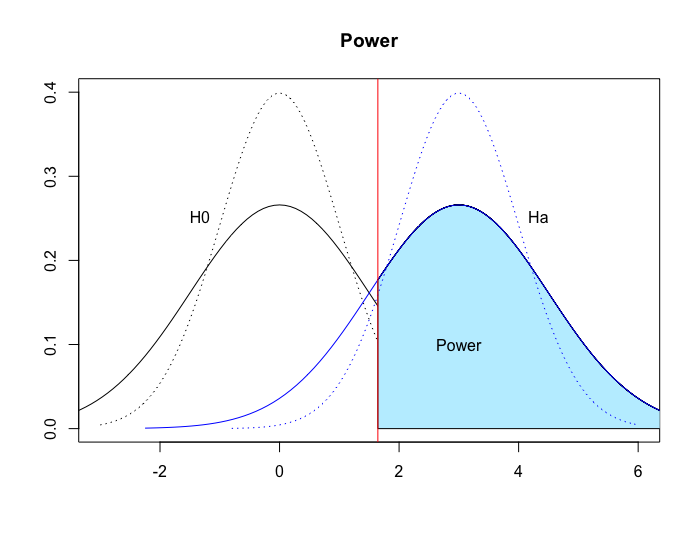
\includegraphics[width=0.9\textwidth]{underpoweredimprecise.png}
\end{frame}

\begin{frame}{Visualizing Underpowered Estimates}{Small Relative Differences}
	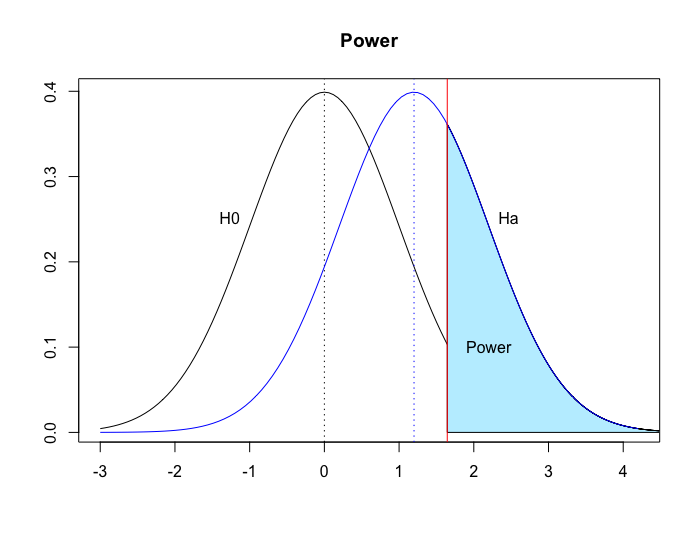
\includegraphics[width=0.9\textwidth]{underpoweredsmalldiff.png}
\end{frame}

\begin{frame}{Spotting Underpowered Estimates}
	How can we avoid underpowered estimates? There are two main root causes:

	\begin{itemize}
		\item Imprecise estimates
			\begin{itemize}
		      	\item Low precision/high variance
		      	\item Large standard errors interpreted as ``no effect''
			\end{itemize}
		\item Small relative differences between $\theta_0$ and $\theta_a$
			\begin{itemize}
		      	\item Precise estimates can detect small relative differences
		      	\item Imprecise estimates require large relative differences to detect the truth. 
			\end{itemize}
	\end{itemize}
			 
	Watch for imprecise estimates! They are often interpreted as a true result when really they are underpowered. %Example: refugee inflows and crime.
\end{frame}



	
\begin{frame}{Importance of Power}
	Sometimes in the economic literature, researchers will state results that don't overturn the null.  Should these results always be believed? Well... maybe not.
	
	\vspace{10mm}

	Sometimes that magnitude of the true value required to produce an acceptable level of power (say, 80\%) is so high it's unreasonable.   That means that even if you repeatedly sampled, you are unlikely to identify the true effect.
\end{frame}
		 

\begin{frame}{Importance of Power}
	This is a common problem in statistics that most people (even economists) often overlook.   Displaying these results without some mention of power is misleading. Some researchers have shown half of all economics research areas have as much as 90\% of results that are underpowered (and therefore suspect).\footnote{\tiny Ioannidis, Stanley \& Doucouliagos, \textit{The Power of Bias in Economics Research} (2017)}
\end{frame}


\begin{frame}{Example: Underpowered Estimates}
	Suppose from 10 observations you estimate that raising the minimum wage by 1\% would lead to only a 0.1\% decline in employment on average with a standard deviation of 6\%.   Can you reject the null that employment wouldn't decrease at the 5\% significance level?
			 
	\begin{align*} 
		p\text{-value} & = Pr(\bar{X} < -0.1 \ \vert \ \mu=0) = Pr\left(\frac{\bar{X} - \mu_0}{\sigma / \sqrt{n}} < \frac{-0.1 - 0}{6/\sqrt{10}}\right) \\
		& = Pr(Z < -0.053) = 0.479      
	\end{align*}
			 
	Since $p$-value $\nleqslant \alpha$, we conclude there is not enough evidence to say that average employment reduction is not 0\% (no effect of minimum wage).
\end{frame}

\begin{frame}{Example: Underpowered Estimates}
	Great news! Raising the minimum wage has no statistically discernible effect on employment, right?   Well.. hold on... If there is an effect on employment our statistic may be too underpowered to detect it.  		 
	Let's calculate the power of this test....
\end{frame}


\begin{frame}{Example: Underpowered Estimates}
	Calculate power by P($\bar{X} \in R \ \vert \ \mu_0$ false)
	 
	This means we must first calculate the rejection region
	 If $\alpha=.05$, then the rejection region is $R = \{ \bar{X} \ \vert \ \bar{X} < -3.12 \}$. 
\end{frame}

\begin{frame}{Example: Underpowered Estimates}
	Let's assume a reasonable negative impact on employment of 0.5\%. (So we're assuming the true $\mu=-0.5$). \\

	Then the power is:
			 
	\[
		P(\text{Reject }H_0 \ \vert \ \mu=-0.5)
	\]
	\[
		P(\bar{X}<-3.12 \ \vert \ \mu=-0.5) = P(Z < \frac{-3.12-(-0.5)}{6/\sqrt{10}})
	\]
	\[
		= P(Z < -1.38) \approx 0.0836  
	\]
	
	Our power to detect a measurable effect is a measly 8.4\%! How did this paper get published anyway?!
\end{frame}

	







\end{document}